Next we explore a collective algorithm that tries to solve the game for all configurations as much as possible, then split the configurations in two sets, create subgames using those two configuration sets and recursively repeat the process. Specifically we try to find vertices that are won by the same player for all configurations in $\mathfrak{C}$, if we have a vertex that is won by the same player for all configurations we call such a vertex \textit{pre-solved}. The algorithm tries to recursively increase the set of pre-solved vertices until all vertices are either pre-solved or only 1 configuration remains. Pseudo code is presented in algorithm \ref{alg_IncPreSolveBasic}. The algorithm is based around finding sets $P_0$ and $P_1$, furthermore we want to find these sets in an efficient manner such that the algorithm doesn't spend time finding vertices that are already pre-solved. Finally when there is only 1 configuration left we want an algorithm that solves the parity game $G_{|c}$ in an efficient manner by using the vertices that are pre-solved.

\begin{algorithm}
	\caption{$\textsc{IncPreSolve}(G = (V,V_0,V_1, E, \Omega, \mathfrak{C}, \theta), P_0,P_1)$}\label{alg_IncPreSolveBasic}
	\begin{algorithmic}[1]
		\If{$|\mathfrak{C}| = 1$}
		\State $\{c\} \gets \mathfrak{C}$
		\State $(W'_0,W'_1) \gets $ solve $G_{|c}$ using $P_0$ and $P_1$
		\State \Return $(\mathfrak{C} \times W'_0, \mathfrak{C} \times W'_1)$
		\EndIf
		\State $P'_0 \gets$ find vertices won by player $0$ for all configuration in $\mathfrak{C}$
		\State $P'_1 \gets$ find vertices won by player $1$ for all configuration in $\mathfrak{C}$
		\If{$P'_0 \cup P'_1 = V$}
		\State \Return $(\mathfrak{C} \times P'_0, \mathfrak{C} \times P'_1)$
		\EndIf
		\State $\mathfrak{C}^a, \mathfrak{C}^b \gets $ partition $\mathfrak{C}$ in non-empty parts
		\State $(W_0^a, W_1^a) \gets \textsc{IncPreSolve}(G \cap \mathfrak{C}^a, P'_0,P'_1)$
		\State $(W_0^b, W_1^b) \gets \textsc{IncPreSolve}(G \cap \mathfrak{C}^b, P'_0,P'_1)$
		\State $W_0 \gets W_0^a \cup W_0^b$
		\State $W_1 \gets W_1^a \cup W_1^b$
		\State \Return $(W_0,W_1)$
	\end{algorithmic}
\end{algorithm}
The subgames created are based on a set of configurations, we define the subgame operator as follows:
\begin{definition}
	Given VPG $G = (V,V_0,V_1,E,\Omega,\mathfrak{C},\theta)$ and non-empty set $\mathfrak{X} \subseteq \mathfrak{C}$ we define the subgame $G \cap \mathfrak{X} = (V,V_0,V_1,E',\Omega,\mathfrak{C}', \theta')$ such that
	\begin{itemize}
		\item $\mathfrak{C}' =\mathfrak{C} \cap \mathfrak{X}$,
		\item $\theta'(e) = \theta(e) \cap \mathfrak{C}'$ and
		\item $E' = \{ e \in E\ |\ \theta'(e) \neq \emptyset \}$.
	\end{itemize}
\end{definition}
VPGs are total, meaning that for every configuration and every vertex there is an outgoing edge from that vertex admitting that configuration. In subgames the set of configurations is restricted and only edge guards and edges are removed for configurations that fall outside the restricted set, therefore we still have totality. Furthermore it is trivial to see that every projection $G_{|c}$ is equal to $(G \cap \mathfrak{X})_{|c}$ for any $c \in \mathfrak{C} \cap \mathfrak{X}$.

Finally the subgame operator is associative, meaning $(G \cap \mathfrak{X}) \cap \mathfrak{X}' = G \cap (\mathfrak{X} \cap \mathfrak{X}') = G \cap \mathfrak{X} \cap \mathfrak{X}'$.

\subsection{Finding $P_0$ and $P_1$}
We can find $P_0$ and $P_1$ by using \textit{pessimistic} parity games; a pessimistic PG is a parity game created from a VPG for a player $\alpha \in \{0,1\}$ such that the PG allows all edges that player $\overline{\alpha}$ might take but only allows edges for $\alpha$ when that edge admits all the configurations in $\mathfrak{C}$.
\begin{definition}
	\label{def_pess_game}
	Given VPG $G = (V,V_0,V_1,E,\Omega, \mathfrak{C},\theta)$, we can create pessimistic PG $G_{\triangleright\alpha}$ for player $\alpha \in \{0,1\}$. We have	
	\[ G_{\triangleright\alpha} = \{V,V_0,V_1,E',\Omega \} \]
	such that
	\[ E' = \{ (v,w) \in E\ |\ v \in V_{\overline{\alpha}} \vee \theta(v,w) = \mathfrak{C} \} \]
\end{definition}


Note that pessimistic parity games are not necessarily total. A play in a PG that is not total might result in a finite path, in such a case the player that can't make a move looses the play.

When solving a pessimistic PG $G_{\triangleright\alpha}$ we get winning sets $W_0,W_1$, every vertex in $W_\alpha$ is winning for player $\alpha$ in $G$ played for any configuration, as shown in the following theorem.
\begin{theorem}
	\label{the_pess_is_winning_for_all_conf}
	Given:
	\begin{itemize}
		\item VPG $G = (V,V_0,V_1,E,\Omega,\mathfrak{C},\theta)$,
		\item configuration $c \in \mathfrak{C}$,
		\item winning sets $W_0^c, W_1^c$ for game $G$,
		\item player $\alpha \in \{0,1\}$ and
		\item pessimistic PG $G_{\triangleright\alpha}$ with winning sets $P_0$ and $P_1$
	\end{itemize}
	we have $P_\alpha \subseteq W_\alpha^c$.
	\begin{proof}
		Player $\alpha$ has a strategy in game $G_{\triangleright\alpha}$ such that vertices in $P_\alpha$ are won. We will show that this strategy can also be applied to game $G_{|c}$ to win the same or more vertices.
		
		First we observe that any edge that is taken by player $\alpha$ in game $G_{\triangleright\alpha}$ can also be taken in game $G_{|c}$ so player $\alpha$ can play the same strategy in game $G_{|c}$.
		
		For player $\overline{\alpha}$ there are possibly edges that can be taken in $G_{\triangleright\alpha}$ but can't be taken in $G_{|c}$, in such a case player $\overline{\alpha}$'s choices are limited in game $G_{|c}$ compared to $G_{\triangleright\alpha}$ so if player $\overline{\alpha}$ can't win a vertex in $G_{\triangleright\alpha}$ then he/she can't win that vertex in $G_{|c}$.
		
		We can conclude that applying the strategy from game $G_{\triangleright\alpha}$ in game $G_{|c}$ for player $\alpha$ wins the same or more vertices.
	\end{proof}
\end{theorem}
Figure \ref{fig:VPG2PPGs} shows an example VPG with corresponding pessimistic games, after solving the pessimistic games we find $P_0 = \{v_2\}$ and $P_1 = \{v_0\}$.
\begin{figure}[h]
	\centering
	\begin{subfigure}{1\textwidth}
		\centering
		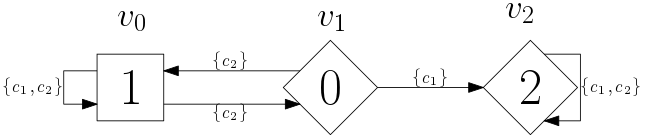
\includegraphics[scale=0.4]{Examples/PPG/VPG}
		\caption{VPG $G$ consisting of 2 configurations}
	\end{subfigure}\\
	\begin{subfigure}{1\textwidth}
		\centering
		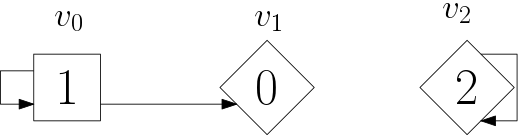
\includegraphics[scale=0.4]{Examples/PPG/P0}
		\caption{Pessimistic game $G_{\triangleright0}$}
	\end{subfigure}\\
	\begin{subfigure}{1\textwidth}
		\centering
		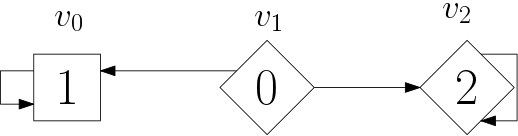
\includegraphics[scale=0.4]{Examples/PPG/P1}
		\caption{Pessimistic game $G_{\triangleright1}$}
	\end{subfigure}
	\caption{A VPG with its corresponding pessimistic games}
	\label{fig:VPG2PPGs}
\end{figure}
\subsubsection{Pessimistic subgames}
Vertices in winning set $P_\alpha$ for $G_{\triangleright\alpha}$ are also winning for player $\alpha$ in pessimistic subgames of $G$, as shown in the following lemma.
\begin{lemma}
	\label{lem_pessimistic_subgames}
	Given:
	\begin{itemize}
		\item VPG $G = (V,V_0,V_1,E,\Omega, \mathfrak{C},\theta)$,
		\item $P_0$ being the winning set of game $G_{\triangleright0}$ for player $0$,
		\item $P_1$ being the winning set of game $G_{\triangleright1}$ for player $1$,
		\item non-empty set $\mathfrak{X} \subseteq \mathfrak{C}$,
		\item player $\alpha \in \{0,1\}$ and
		\item winning sets $Q_0,Q_1$ for game $(G \cap \mathfrak{X})_{\triangleright\alpha}$
	\end{itemize}
	we have
	\[ P_0 \subseteq Q_0 \]
	\[ P_1 \subseteq Q_1 \]
	\begin{proof}
		
		Let edge $(v,w)$ be an edge in game $G_{\triangleright\alpha}$ with $v \in V_\alpha$. Edge $(v,w)$ admits all configuration in $\mathfrak{C}$ so it also admits all configuration in $\mathfrak{C} \cap \mathfrak{X}$, therefore we can conclude that edge $(v,w)$ is also an edge of game $(G\cap \mathfrak{X})_{\triangleright\alpha}$.
		
		Let edge $(v,w)$ be an edge in game $(G \cap \mathfrak{X})_{\triangleright\alpha}$ with $v \in V_{\overline{\alpha}}$. The edge admits some configuration in $\mathfrak{C} \cap \mathfrak{X}$, this configuration is also in $\mathfrak{C}$ so we can conclude that edge $(v,w)$ is also an edge of game $G_{\triangleright\alpha}$.
		
		We have concluded that game $(G \cap \mathfrak{X})_{\triangleright\alpha}$ has the same or more edges for player $\alpha$ as game $G_{\triangleright\alpha}$ and the same or less edges for player $\overline{\alpha}$. Therefore we can conclude that any vertex won by player $\alpha$ in $G_{\triangleright\alpha}$ is also won by $\alpha$ in game $(G \cap \mathfrak{X})_{\triangleright\alpha}$, ie. $P_\alpha \subseteq Q_\alpha$.
		
		
		Let $v \in P_{\overline{\alpha}}$, using theorem \ref{the_pess_is_winning_for_all_conf} we find that $v$ is winning for player $\overline{\alpha}$ in $G_{|c}$ for any $c \in \mathfrak{C}$. Because projections of subgames are the same as projections of the original game we can conclude that $v$ is winning for player $\overline{\alpha}$ in $(G \cap \mathfrak{X})_{|c}$ for any $c \in \mathfrak{C} \cap \mathfrak{X}$.
		
		Assume $v \notin Q_{\overline{\alpha}}$ then $v \in Q_{\alpha}$ and using theorem \ref{the_pess_is_winning_for_all_conf} we find that $v$ is winning for player $\alpha$ in $(G \cap \mathfrak{X})_{|c}$ for any $c \in \mathfrak{C} \cap \mathfrak{X}$. This is a contradiction so we can conclude $v \in Q_{\overline{\alpha}}$ and therefore $P_{\overline{\alpha}} \subseteq Q_{\overline{\alpha}}$.
	\end{proof}
\end{lemma}
\subsection{Algorithm}
In order to find $P_0$ and $P_1$ we need to solve a pessimistic parity game, specifically we want to solve a parity game that uses the vertices that are already pre-solved to efficiently solve the parity game. Note that when there is 1 configuration left we need a similar algorithm. In algorithm \ref{alg_IncPreSolve} we present the \textsc{IncPreSolve} algorithm using pessimistic parity games. The algorithm uses a \textsc{Solve} algorithm for solving parity games using the pre-solved vertices. First we show the correctness of the \textsc{IncPreSolve} algorithm, later we explore an appropriate \textsc{Solve} algorithm.
\begin{algorithm}
	\caption{$\textsc{IncPreSolve}(G = (V,V_0,V_1, E, \Omega, \mathfrak{C}, \theta), P_0,P_1)$}\label{alg_IncPreSolve}
	\begin{algorithmic}[1]
		\If{$|\mathfrak{C}| = 1$}
		\State $\{c\} \gets \mathfrak{C}$
		\State $(W'_0,W'_1) \gets \textsc{Solve}(G_{|c}, P_0,P_1)$
		\State \Return $(\mathfrak{C} \times W'_0, \mathfrak{C} \times W'_1)$
		\EndIf
		\State $(P'_0,-) \gets \textsc{Solve}(G_{\triangleright0}, P_0, P_1)$
		\State $(-,P'_1) \gets \textsc{Solve}(G_{\triangleright1}, P_0, P_1)$
		\If{$P'_0 \cup P'_1 = V$}
		\State \Return $(\mathfrak{C} \times P'_0, \mathfrak{C} \times P'_1)$
		\EndIf
		\State $\mathfrak{C}^a, \mathfrak{C}^b \gets $ partition $\mathfrak{C}$ in non-empty parts
		\State $(W_0^a, W_1^a) \gets \textsc{IncPreSolve}(G \cap \mathfrak{C}^a, P'_0,P'_1)$
		\State $(W_0^b, W_1^b) \gets \textsc{IncPreSolve}(G \cap \mathfrak{C}^b, P'_0,P'_1)$
		\State $W_0 \gets W_0^a \cup W_0^b$
		\State $W_1 \gets W_1^a \cup W_1^b$
		\State \Return $(W_0,W_1)$
	\end{algorithmic}
\end{algorithm}

A \textsc{Solve} algorithm must correctly solve a game as long as the sets $P_0$ and $P_1$ are in fact vertices that are won by player $0$ and $1$ respectively. We prove that this is the case in the \textsc{IncPreSolve} algorithm.
\begin{theorem}
	Given VPG $\hat{G}$. For every $\textsc{Solve}(G,P_0,P_1)$ that is invoked during $\textsc{IncPreSolve}(\hat{G},\emptyset,\emptyset)$ we have winning sets $W_0,W_1$ for game $G$ for which the following holds:
	\[ P_0 \subseteq  W_0 \]
	\[ P_1 \subseteq  W_1 \]
	\begin{proof}
		When $P_0 = \emptyset$ and $P_1 = \emptyset$ the theorem holds trivially. So we will start the analyses after the first recursion. 
		
		After the first recursion the game is $\hat{G} \cap \mathfrak{X}$ with $\mathfrak{X}$ being either $\mathfrak{C}^a$ or $\mathfrak{C}^b$. The set $P_0$ is the winning set for player $0$ for game $\hat{G}_{\triangleright0}$ and the set $P_1$ is the winning set for player $1$ for game $\hat{G}_{\triangleright1}$. In the next recursion the game is $\hat{G} \cap \mathfrak{X} \cap \mathfrak{X}'$ with $P_0$ being the winning set for player $0$ in game $(\hat{G} \cap \mathfrak{X})_{\triangleright0}$ and $P_1$ being the winning set for player $1$ in game $(\hat{G} \cap \mathfrak{X})_{\triangleright1}$. In general, after the $k$th recursion, with $k > 0$, the game is of the form  $(\hat{G} \cap \mathfrak{X}^0 \cap \dots \cap \mathfrak{X}^{k-1}) \cap \mathfrak{X}^k$. Furthermore $P_0$ is the winning set for player $0$ for game $(\hat{G} \cap \mathfrak{X}^0 \cap \dots \cap \mathfrak{X}^{k-1})_{\triangleright0}$ and $P_1$ is the winning set for player $1$ for game $(\hat{G} \cap \mathfrak{X}^0 \cap \dots \cap \mathfrak{X}^{k-1})_{\triangleright1}$.
		
		Next we inspect the three places \textsc{Solve} is invoked:
		\begin{enumerate}
			\item Consider the case where there is only one configuration in $\mathfrak{C}$ (line 1-5). Because $P_0$ is the winning set for player $0$ for game $(\hat{G} \cap \mathfrak{X}^0 \cap \dots \cap \mathfrak{X}^{k-1})_{\triangleright0}$ the vertices in $P_0$ are won by player $0$ in game $G_{|c}$ for all $c \in \mathfrak{X}^0 \cap \dots \cap \mathfrak{X}^{k-1}$ (using theorem \ref{the_pess_is_winning_for_all_conf}). This includes the one element in $\mathfrak{C}$. So we can conclude $P_0 \subseteq W_0$ where $W_0$ is the winning set for player $0$ in game $G_{|c}$ where $\{c\} = \mathfrak{C}$.
			
			Similarly for player $1$ we can conclude $P_1 \subseteq W_1$ and the theorem holds in this case.
			\item On line $6$ the game $G_{\triangleright0}$ is solved with $P_0$ and $P_1$. Because $G = \hat{G} \cap \mathfrak{X}^0 \cap \dots \cap \mathfrak{X}^{k-1} \cap \mathfrak{X}^k$ and $P_0$ is the winning set for player $0$ for game $(\hat{G} \cap \mathfrak{X}^0 \cap \dots \cap \mathfrak{X}^{k-1})_{\triangleright0}$ and $P_1$ is the winning set for player $1$ for game $(\hat{G} \cap \mathfrak{X}^0 \cap \dots \cap \mathfrak{X}^{k-1})_{\triangleright1}$ we can apply lemma \ref{lem_pessimistic_subgames} to conclude that the theorem holds in this case.
			\item On line $7$ we apply the same reasoning and lemma to conclude that the theorem holds in this case.
		\end{enumerate}
	\end{proof}
\end{theorem}

Next we prove the correctness of the algorithm, assuming the correctness of the \textsc{Solve} algorithm.
\begin{theorem}
	%TODO hat notatie
	Given VPG $\hat{G} = (\hat{V},\hat{V}_0,\hat{V}_1,\hat{E},\hat{\Omega},\mathfrak{C},\theta)$ and $(W_0,W_1) = \textsc{IncPreSolve}(\hat{G},\emptyset,\emptyset)$. For every configuration $c \in \mathfrak{C}$ and winning sets $\hat{W}_0^c, \hat{W}_1^c$ for game $\hat{G}$ player for $c$ it holds that:
	\[ (c,v) \in W_0 \iff v \in \hat{W}_0^c \]
	\[ (c,v) \in W_1 \iff v \in \hat{W}_1^c \]
	\begin{proof}
		We will prove the theorem by applying induction on $\mathfrak{C}$.
		
		\textbf{Base} $|\mathfrak{C}| = 1$, when there is only one configuration, being $c$, then the algorithm solves game $G_{|c}$. The product of the winning sets and $\{c\}$ is returned, so the theorem holds.
		
		\textbf{Step} Consider $P_0'$ and $P_1'$ as calculated in the algorithm (line 6-7). By theorem \ref{the_pess_is_winning_for_all_conf} all vertices in $P_0'$ are won by player $0$ in game $G_{|c}$ for any $c \in \mathfrak{C}$, similarly for $P_1'$ and player $1$.
		
		If $P_0' \cup P_1' = V$ then the algorithm returns $(\mathfrak{C} \times P_0',\mathfrak{C} \times P_1')$. In which case the theorem holds because there are no configuration vertex combinations that are not in either winning set and theorem \ref{the_pess_is_winning_for_all_conf} proves the correctness.
		
		If $P_0' \cup P_1' \neq V$ then we have winning sets $(W_0^a, W_1^a)$ for which the theorem holds (by induction) for game $G \cap \mathfrak{C}^a$ and $(W_0^b, W_1^b)$ for which the theorem holds (by induction) for game $G \cap \mathfrak{C}^b$. The algorithm returns $(W_0^a \cup W_0^b, W_1^a \cup W_1^b)$. Since $\mathfrak{C}^a \cup \mathfrak{C}^b = \mathfrak{C}$ all vertex configuration combinations are in the winning sets and the correctness follows from induction.
	\end{proof}
\end{theorem}

\subsection{A parity game algorithm using pre-solved vertices}
The fixed-point iteration algorithm can be used to solve parity games using pre-solved vertices. First recall the fixed-point formula to calculate $W_0$:
\[ S(G = (V,V_0,V_1,E,\Omega)) = \nu Z_{d-1}. \mu Z_{d-2}. \dots . \nu Z_0. F_0(Z_{d-1},\dots,Z_0) \]

Let $G$ be a PG and let sets $P_0$ and $P_1$ be such that vertices in $P_0$ are won by player $0$ and vertices in $P_1$ are won by player $1$. We can fixed-point iterate $S(G)$ to calculate $W_0$, we know that $W_0$ is bounded by $P_0$ and $P_1$, specifically we have
\[ P_0 \subseteq W_0 \subseteq V\backslash P_1\]
We can use this restriction to efficiently iterate $S(G)$. If no bounds are know we would iterate fixed-point formula $\nu Z_{d-1}\dots$ by starting at $Z_{d-1}^0 = V$ which is the largest value possible, however given the bounds we can start our iterations of greatest fixed-point variables at $V\backslash P_1$ and start our iterations of least fixed-point variables at $P_0$. The following lemma's and theorems prove this.
\begin{lemma}
	\label{lem_fixpoint_bounds_nu}
	Given
	\begin{itemize}
		\item A complete lattice $\langle 2^A, \subseteq \rangle$,
		\item monotonic function $f : 2^A \rightarrow 2^A$ and
		\item $R^\bot \subseteq A$ and $R^\top \subseteq A$ such that $R^\bot \subseteq \nu X. f(X) \subseteq R^\top$
	\end{itemize}
	we iterate $X$ by starting with $X^0 = R^\top$. For any $i \geq 0$ it holds that
	\[ R^\bot \subseteq f(X^i) \subseteq R^\top \]
	\begin{proof}
		Assume $R^\bot \supset f(X^i)$. By fixed-point iteration we have $\nu X.f(X) = \cap_{j\geq0} X^j$, so we find $R^\bot \supset \nu X.f(x)$ which is a contradiction so $R^\bot \subseteq f(X^i)$.
		
		Assume $f(X^i) \supset R^\top$. Because of monotonicity we find $X^i \subseteq R^\top$ and therefore $f(X^i) \supset R^\top \supseteq X^i$. Using the Knaster-Tarski theorem (\ref{the_knaster_tarski}) we can conclude that the greatest fixed-point of $f(X)$ is larger than $f(X^i)$, so we find $\nu X.f(X) \supset R^\top$ which is a contradiction so $f(X^i) \subseteq R^\top$.
	\end{proof}
\end{lemma}

\begin{lemma}
	\label{lem_fixpoint_bounds_mu}
	Given
	\begin{itemize}
		\item A complete lattice $\langle 2^A, \subseteq \rangle$,
		\item monotonic function $f : 2^A \rightarrow 2^A$ and
		\item $R^\bot \subseteq A$ and $R^\top \subseteq A$ such that $R^\bot \subseteq \mu X. f(X) \subseteq R^\top$
	\end{itemize}
	we iterate $X$ by starting with $X^0 = R^\bot$. For any $i \geq 0$ it holds that
	\[ R^\bot \subseteq f(X^i) \subseteq R^\top \]
\end{lemma}

\begin{theorem}
	\label{the_FPITE_starting}
	Given PG $G = (V,V_0,V_1,E,\Omega)$ with $P_0$ and $P_1$ such that vertices  in $P_0$ are won by player $0$ in game $G$ and vertices in $P_1$ are won by player $1$ in game $G$ we can iterate the fixed-point variables by starting at $P_0$ for least fixed-points and starting at $V \backslash P_1$ for greatest fixed-points.
	\begin{proof}
		Let $f(Z_{d-1}) = \mu Z_{d-2}\dots\nu Z_0.F_0(Z_{d-1},\dots,Z_0)$. Because $\nu Z_{d-1}.f(Z_{d-1})$ calculates $W_0$ we know $P_0 \subseteq \nu Z_{d-1}.f(Z_{d-1}) \subseteq V \backslash P_1$ so we can start the fixed-point iteration at $Z_{d-1}^0 = V\backslash P_1$. Using lemma \ref{lem_fixpoint_bounds_nu} we find for any $i \geq 0$ we have $P_0 \subseteq f(Z_{d-1}^i) \subseteq V \backslash P_1$.
		
		Let $g(Z_{d-2}) = \nu Z_{d-3} \dots \nu Z_0. F_0(Z_{d-1}^i,Z_{d-2},\dots,Z_0)$. We found $P_0 \subseteq f(Z_{d-1}^i) \subseteq V \backslash P_1$, therefore we have $P_0 \subseteq \mu Z_{d-2}.g(Z_{d-2})\subseteq V \backslash P_1$ so we can start the fixed-point iteration at $Z_{d-2}^0 = P_0$. Using lemma \ref{lem_fixpoint_bounds_mu} we find that for any $j \geq 0$ we have $P_0 \subseteq g(Z_{d-2}^j) \subseteq V\backslash P_1$.
		
		We can repeat this logic up until $Z_0$ to conclude that the theorem holds.
	\end{proof}
\end{theorem}
We take the fixed-point algorithm presented in \cite{FPITE} and modify it by starting at $P_0$ and $V \backslash P_1$. The pseudo code is presented in algorithm \ref{alg_FPITE}, its correctness follows from \cite{FPITE} and theorem \ref{the_FPITE_starting}.
\begin{algorithm}
	\caption{Fixed-point iteration with $P_0$ and $P_1$}
	\label{alg_FPITE}
	\begin{multicols}{2}
		\begin{algorithmic}[1]
			\Function{FPIter}{$G = (V, V_0, V_1, E, \Omega), P_0, P_1$}
				\For{$i \gets d-1,\dots,0$}
					\State $\textsc{Init}(i)$
				\EndFor
				\Repeat
					\State $Z_0'\gets Z_0$
					\State $Z_0 \gets \textsc{Diamond}() \cup \textsc{Box}()$
					\State $i \gets 0$
					\While{$Z_i=Z_i' \wedge i < d-1$}
						\State $i \gets i+1$
						\State $Z_i' \gets Z_i$
						\State $Z_i \gets Z_{i-1}$
						\State $\textsc{Init}(i-1)$
					\EndWhile
				\Until{$i = d-1 \wedge Z_{d-1} = Z_{d-1}'$}
				\State \Return $(Z_{d-1},V\backslash Z_{d-1})$
			\EndFunction
		\end{algorithmic}\bigskip\bigskip
		\begin{algorithmic}[1]
			\Function{Init}{$i$}
				\State $Z_i \gets P_0$ if $i$ is odd, $V\backslash P_1$ otherwise
			\EndFunction
		\end{algorithmic}\bigskip
		\begin{algorithmic}[1]
			\Function{Diamond}{}
				\State \Return $\{ v \in V_0\ |\ \exists_{w\in V} (v,w) \in E \wedge w \in Z_{\Omega(w)}\}$
			\EndFunction
		\end{algorithmic}\bigskip
		\begin{algorithmic}[1]
			\Function{Box}{}
			\State \Return $\{ v \in V_1\ |\ \forall_{w\in V} (v,w) \in E \implies w \in Z_{\Omega(w)}\}$
			\EndFunction
		\end{algorithmic}
	\end{multicols}
\end{algorithm}

This algorithm is appropriate to use as a \textsc{Solve} algorithm in \textsc{IncPreSolve} since it solves parity games that are not necessarily total and uses $P_0$ and $P_1$.

\subsection{Running time}
We will consider the running time for solving VPG $G = (V,V_0,V_1,E,\Omega,\mathfrak{C},\theta)$ independently and collectively. Let $n$ denote the number of vertices, $e$ the number of edges, $c$ the number of configurations and $d$ the number of distinct priorities.

The fixed-point iteration algorithm without $P_0$ and $P_1$ runs in $O(e*n^d)$ (\cite{FPITE}). We can use this algorithm to solve $G$ independently, ie. solve all the projections of $G$. This gives a time complexity of $O(c*e*n^d)$.

Next we consider the \textsc{IncPreSolve} algorithm for a collective approach, observe that in the worst case we have to split the set of configurations all the way down to individual configurations. We can consider the recursion as a tree where the leafs are individual configurations and at every internal node the set of configurations is split in two. Since in the worst case there are $c$ leaves, there are at most $c-1$ internal nodes. At every internal node the algorithm solves two games and at every leaf the algorithm solves 1 game, so we get $c + 2c - 2 = O(c)$ games that are being solved by \textsc{IncPreSolve}. In the worst case there are no similarities between the configuration in $G$ and at every iteration $P_0$ and $P_1$ are empty. In this case the \textsc{FPIte} algorithm behaves the same as the original algorithm and has a time complexity of $O(e*n^d)$, this gives an overall time complexity of $O(c*e*n^d)$ which is equal to an independent solving approach.